\subsection*{Tasks and concurrency}
A \underline{task} is a set of program instructions, a \underline{process} is an instance of a computer program that
is being executed, and a \underline{thread} is a basic unit of CPU utilization that can exist within a
process. Meaning a thread consists of a program counter, a stack, and a set of registers.\\
Each thread has its own stack, but all threads in a process share the same heap. The stack is
used for storing temporary data that is created and destroyed during the execution of a
function, while the heap is used for storing data that needs to persist beyond the lifetime of
a function.
% \begin{wrapfigure}{r}{0.5\columnwidth}
%     \centering
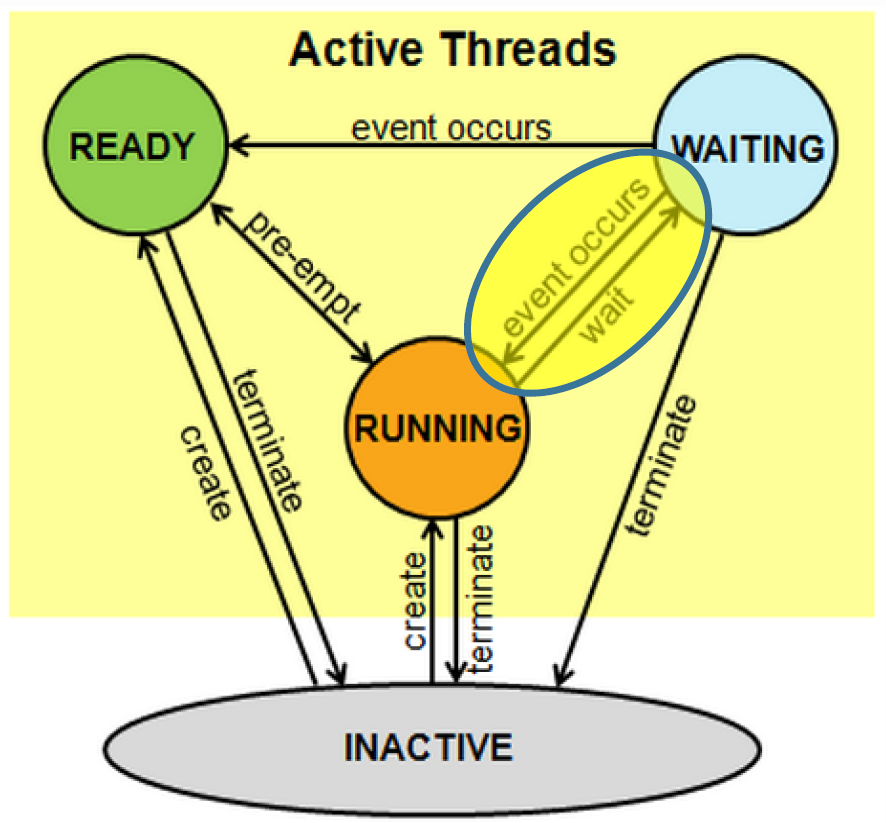
\includegraphics[width=\columnwidth]{images/thread_states.png}
% \end{wrapfigure}
In a multitasking system, the different tasks may compete for shared resources or may wait for
different events to happen. In some cases, a given task may thus enter a Waiting or Blocked state.\\
\underline{Mutex:} only one thread can access a shared resource at a time.
\begin{minted}{c++}
Mutex mtx;
mtx.lock();
//critical section
mtx.unlock();
\end{minted}
\underline{Semaphore:}\\
A semaphore is a synchronization object that controls access to a shared resource by multiple
threads. Unlike a mutex, a semaphore can control access to several shared resources.
\begin{minted}{c++}
Semaphore sem_in {2};
Semaphore sem_out {0};
sem_in.acquire(); //decrement
//critical section
sem_out.release(); //increment
\end{minted}
\underline{Deadlock:}\\
A deadlock is a situation where two or more competing tasks are waiting for each other to
finish, and thus neither ever does.\\
\underline{Queue/Mail:}\\
A queue is a FIFO data structure that can be used to pass messages between tasks.\\